%!TeX ts-program = xelatex
\documentclass[10pt]{IEEEtran}
\usepackage[vmargin=1in, hmargin=1.2in]{geometry}
\usepackage{fontspec}
\usepackage[dvipsnames]{xcolor}
\setmainfont{QTBookmann}
\usepackage{polyglossia}
\usepackage{graphicx}
\usepackage{dirtytalk}
\setdefaultlanguage[variant=mexican]{spanish}
\usepackage{multirow}
\usepackage{amsmath}
\usepackage{pgfplots}
\usepackage{subcaption}
\usepackage{tikz}

\author{%
Brandon Marquez Salazar
}
\title{%
Active Contours Detection---Snake Algorithm---For Amoeba Detection
}
\begin{document}
  \maketitle
  \begin{abstract}
    In the field of pattern recognition there's an interest when it comes to
    object recognition or texture in 3 dimensions, where the third dimension is time.
    The snakes\cite{Kass1988} algorithm is a method which allows us to detect objects based on
    pattern recognition features such as the energy.
    In this experiment we'll test the snakes algorithm implemetnted within 
    \texttt{scikit-image}\cite{scikit-image-active-contours}.
  \end{abstract}

  \section{Introduction}

  In several study fields, the most important thing when trying to solve a classification problem
  from video, sometimes is needed to detect the interest object. In this experiment, our ROI is an
  Amoeba which is moving along the window.

  For this, the snakes algorithm\cite{Kass1988} the method that will help the recognition task.

  \section{Methods}

  For this experiment, the first step is to get the image data, the it'll be preprocessed
  enhancing the image to get better results.
  The enhancement will be done via \textbf{histogram normalization}, \textbf{otsu tresholding}
  and a \textbf{gaussian filter}---this one, during the snake algorithm---. Another option, yet
  abandoned was \textbf{inverting} the gray levels of the image, but it gave more unstable results.

  Several values combinations were tested for the coefficients \texttt{$\alpha$}, \texttt{$\beta$} and
  \texttt{$\gamma$}, \textbf{control point numbers} and \textbf{gaussian $\sigma$}.

  \section{Results}

  As it can be seen in figure \ref{fig:results}, the most interesting behaviour of this algorithm
  can be found when a binarization is used. Aldo, the inversion resulted in rapidly collapsed polynoms.

  \begin{figure}[!h]
    \caption{Results}
    \label{fig:results}
    \centering
    \begin{subfigure}{0.4\linewidth}
      \centering
      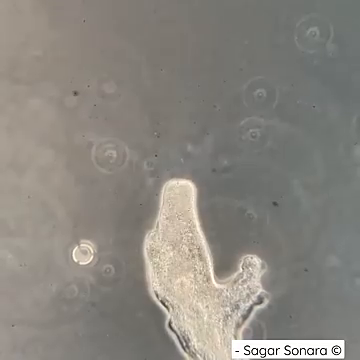
\includegraphics[width=\linewidth]{img/frame0011.png}
      \caption{Original Image}
    \end{subfigure}
    \hfill
    \begin{subfigure}{0.4\linewidth}
      \centering
      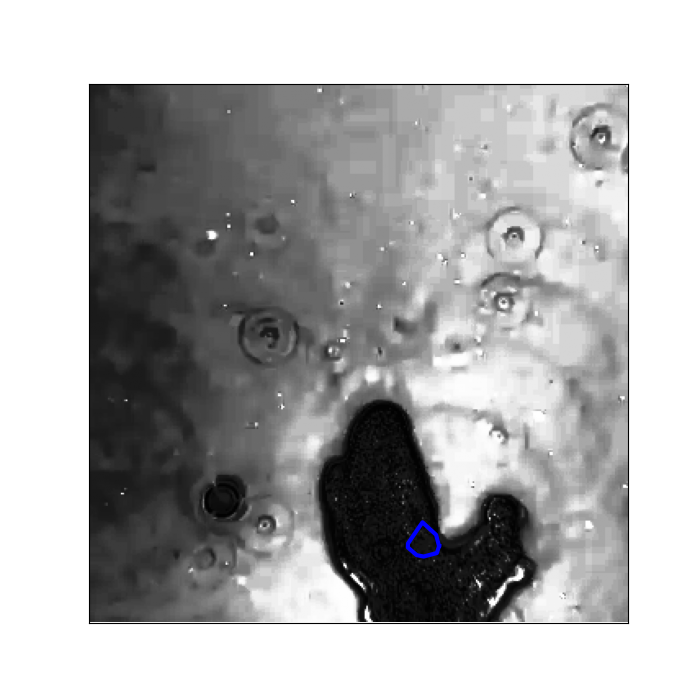
\includegraphics[width=\linewidth]{img/frame0001.png}
      \caption{Enhanced Image Inverted}
    \end{subfigure}
    \begin{subfigure}{0.4\linewidth}
      \centering
      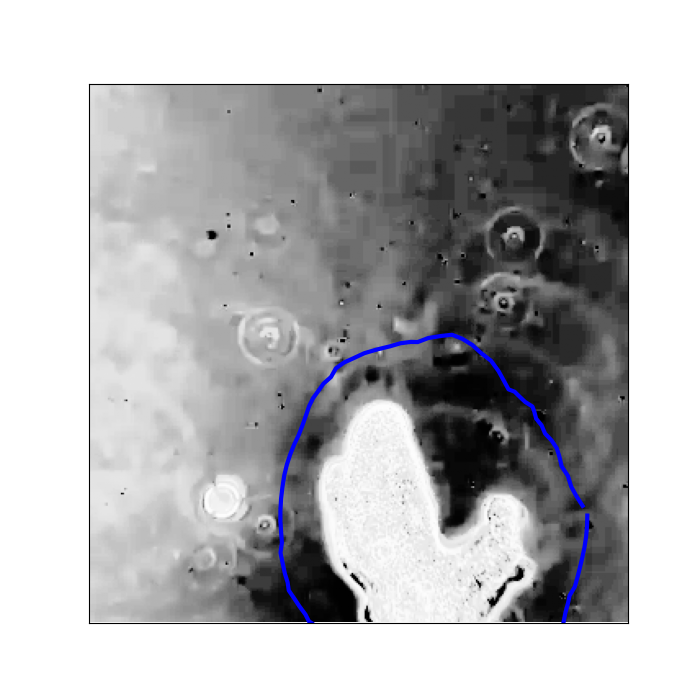
\includegraphics[width=\linewidth]{img/Prueba_0.013a-0.250b-0.010g-200it.png}
      \caption{Enhanced Image}
    \end{subfigure}
    \hfill
    \begin{subfigure}{0.4\linewidth}
      \centering
      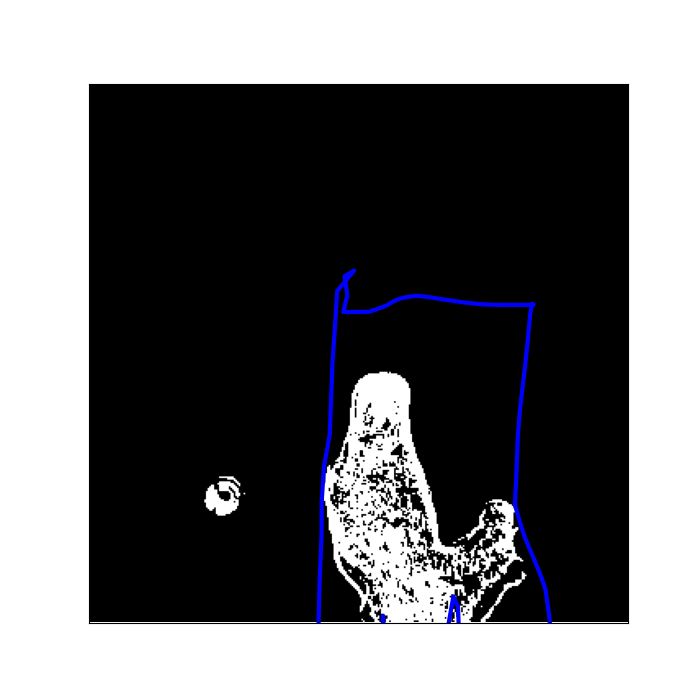
\includegraphics[width=\linewidth]{img/frame0012.png}
      \caption{Binarized image}
    \end{subfigure}
  \end{figure}

  \section{Discussion}
  
  Here is a point to discuss mainly about the parameters used for the best results obtained, 
  and is that there are tons of different combinations, and due time constraints, we could not
  test all of them.
  Also, snakes are a good algorithm but it's not perfect, several tests reflected rapidly collapsed
  polynoms or practically insensitive polynoms.
  It's also important that this approach requires initial conditions which are needed for accuracy, 
  but, even point number can be a totally tricky parameter depending on the problem.

  \section{Conclusions}
  This experiment demosntrates the capabilities of contour detectin of snakes, but, it's needed
  to point out that the main issue is finding the correct hyperparamenters and initial conditions
  for the algorithm to behave correctly.

  Another point is that even the smallest details can alter completely the final polygon behaviour.
  This aims every researcher interested in using this methtod to be aware of this image quality,
  focusing on contrast.

  \section*{References}
  \bibliographystyle{IEEEtran}
  \bibliography{bibliography}
\end{document}
